% Graph-based EGS heat extraction prototype
% build:  python make_figures.py   (figures from data/)
%         pdflatex graph_egs_prototype.tex   (twice)
% speaker notes: uncomment \setbeameroption{show notes on second screen=right}
\documentclass[aspectratio=169,10pt]{beamer}
\usetheme[progressbar=frametitle,numbering=fraction]{metropolis}
\usepackage{amsmath,amssymb}
\usepackage{booktabs}
\usepackage{tikz}
\usetikzlibrary{arrows.meta,positioning}
% \usepackage{pgfpages}\setbeameroption{show notes on second screen=right}

\definecolor{basalt}{HTML}{2B2D42}
\definecolor{ember}{HTML}{D9775C}
\definecolor{blue1}{HTML}{2A78D6}
\definecolor{inkmuted}{HTML}{52514E}
\setbeamercolor{frametitle}{bg=basalt}
\setbeamercolor{progress bar}{fg=ember}
\setbeamercolor{alerted text}{fg=ember!80!black}

\title{Graph-based EGS heat extraction}
\subtitle{Segmented wells, hydraulic fractures, dfnWorks graph flow and an analytic heat-exchange kernel}
\author{Jeffrey Hyman}
\institute{EES-16, Los Alamos National Laboratory}
\date{November 2026}

\tikzset{
  stage/.style={draw=basalt, rounded corners=3pt, fill=white, align=center, font=\small,
                minimum height=1.05cm, text width=2.0cm, inner sep=3pt},
  new/.style={stage, fill=ember!12, draw=ember!80!black},
  flow/.style={-{Stealth[length=2.2mm]}, thick, inkmuted},
}

\begin{document}

\maketitle
\note{A simple, deterministic EGS case built with dfnWorks' own graph tools: two lateral wells, three hydraulic fractures, graph flow between the wells, particle tracking, and an analytic fracture-rock heat exchange kernel that turns each particle path into a cooling curve. Along the way, three inconsistencies in dfnWorks' graph flow and transport were found and fixed on this branch.}

% ------------------------------------------------------------------
\begin{frame}{What this prototype is}
\begin{columns}[T]
\column{0.52\textwidth}
\textbf{Goal}: produced temperature and heat rate for an EGS doublet from the DFN alone: no mesh and no PFLOTRAN run.

\medskip
\textbf{Approach}
\begin{itemize}
  \item native dfnWorks calls only: \texttt{add\_user\_fract}, \texttt{create\_graph}, \texttt{add\_fracture\_source/target}, \texttt{run\_graph\_flow}, \texttt{run\_graph\_transport}
  \item one simple, deterministic geometry we can reason about by hand
  \item thermal step: per-particle analytic kernel (heat as a solute)
\end{itemize}
\column{0.44\textwidth}
\textbf{Replaces} the \texttt{pydfnworks.thermal} wrappers \texttt{add\_hydraulic\_fractures} and \texttt{graph\_flow\_for\_rate}, which repeated what dfnWorks already does.

\medskip
\textbf{Code}
\begin{itemize}\small
  \item \texttt{EGS\_scripts/graph\_based}: \texttt{driver\_v1.py}, \texttt{helper\_functions.py}, \texttt{plot\_results.py}
  \item \texttt{hymanjd/dfnWorks}, branch \texttt{feature/thermal-mpf-surrogate}: graph flow and transport fixes
\end{itemize}
\end{columns}
\note{The earlier thermal package wrapped dfnWorks calls in its own functions, one to place hydraulic fractures and one to solve flow at a target rate. This prototype drops those and uses dfnWorks directly, on a case simple enough that every number can be checked by hand. The thermal step is unchanged in spirit: graph particle tracking gives every flow path, and an analytic kernel converts each path into a cooling curve.}
\end{frame}

% ------------------------------------------------------------------
\begin{frame}{Geometry}
\centering
\includegraphics[width=0.84\textwidth]{figs/geometry.pdf}

\footnotesize
\begin{columns}[T]
\column{0.5\textwidth}
\begin{itemize}
  \item two laterals at $y=\pm 50$\,m, each 23 overlapping 20\,m $\times$ 4\,m segments (2\,m overlap)
  \item segments alternate normals $(0,0,1)$ and $(0,1,0)$: an X cross-section; neighbours cross along the axis
\end{itemize}
\column{0.46\textwidth}
\begin{itemize}
  \item 3 HFs at $x=-100,0,100$\,m (radius 70\,m, aspect 2), each cutting both laterals
  \item injection and production: the $-x$ end segments of the two wells
\end{itemize}
\end{columns}
\note{Each well is a chain of short rectangles rather than one long strip, so the graph resolves flow along the well. Coplanar overlapping polygons do not intersect in dfnGen, so neighbouring segments alternate between a horizontal and a vertical plane; both contain the well axis and cross along it over the 2 m overlap. The chain start is chosen so every hydraulic fracture is at least 4 m from an overlap, which avoids triple intersections. dfnGen inserts user polygons before ellipses, so the injection well is fractures 1 to 23, the production well 24 to 46 and the HFs 47 to 49. Injection and production are both at the minus-x end, on different wells, so water must cross an HF to get from one to the other.}
\end{frame}

% ------------------------------------------------------------------
\begin{frame}{Workflow}
\centering
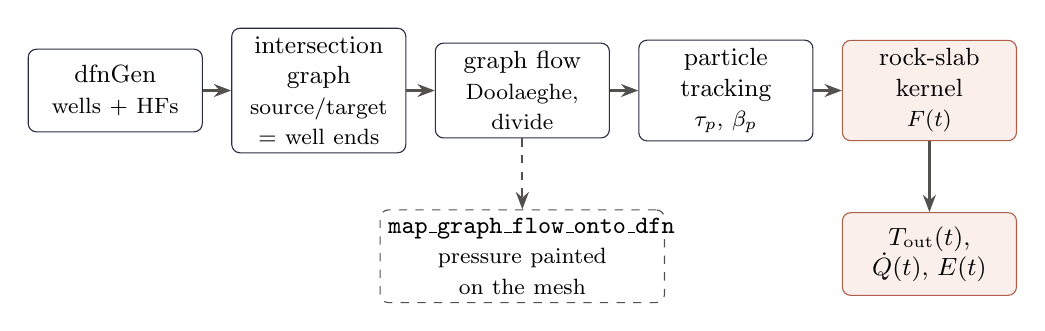
\begin{tikzpicture}[node distance=0.36cm]
  \node[stage] (gen) {dfnGen\\ \footnotesize wells + HFs};
  \node[stage, right=of gen] (graph) {intersection graph\\ \footnotesize source/target = well ends};
  \node[stage, right=of graph] (flow) {graph flow\\ \footnotesize Doolaeghe, divide};
  \node[stage, right=of flow] (trans) {particle tracking\\ \footnotesize $\tau_p$, $\beta_p$};
  \node[new, right=of trans] (heat) {rock-slab kernel\\ \footnotesize $F(t)$};
  \draw[flow] (gen) -- (graph);
  \draw[flow] (graph) -- (flow);
  \draw[flow] (flow) -- (trans);
  \draw[flow] (trans) -- (heat);
  \node[new, below=0.9cm of heat] (out) {$T_\mathrm{out}(t)$, $\dot Q(t)$, $E(t)$};
  \draw[flow] (heat) -- (out);
  \node[stage, below=0.9cm of flow, text width=3.4cm, draw=inkmuted, dashed] (paint) {\texttt{map\_graph\_flow\_onto\_dfn}\\ \footnotesize pressure painted on the mesh};
  \draw[flow, dashed] (flow) -- (paint);
\end{tikzpicture}

\vspace{0.5cm}
\small
\begin{tabular}{@{}ll@{}}
\textcolor{basalt}{$\blacksquare$} existing dfnWorks & \textcolor{ember}{$\blacksquare$} thermal step (\texttt{helper\_functions.py}) \\
\end{tabular}
\note{Left to right: dfnGen builds the 49 fractures; the intersection graph's source and target are re-pointed to the end segments of the two wells with add\_fracture\_source and add\_fracture\_target; graph flow solves steady flow with the Doolaeghe conductance; graph particle tracking, purely advective, records each particle's travel time and exchange integral; the rock-slab kernel turns those into the cooled fraction of produced water, and from that the produced temperature, heat rate and cumulative heat. The flow pressure is also painted onto the DFN mesh for visual checks.}
\end{frame}

% ------------------------------------------------------------------
\begin{frame}{Graph flow: one conductance for pressure, flow and velocity}
\begin{columns}[T]
\column{0.5\textwidth}
Doolaeghe et al.\ (2020) size-aware conductance with the multiple-paths correction ($n_i$ intersections on fracture $i$):
\[ \hat C_e = \frac{C_e}{n_i - 1} \]
Pressures solve the weighted graph Laplacian. Edge flow, area and velocity now all follow from $\hat C_e$:
\[ Q_e = \frac{\hat C_e\,\Delta p_e}{\mu}, \qquad A_e = \frac{\hat C_e\,L_e}{k_e} = b_e W_e \]
\[ v_e = \frac{Q_e}{A_e} = \frac{k_e}{\mu}\,\frac{\Delta p_e}{L_e} \]
\column{0.46\textwidth}
\textbf{Before}
\begin{itemize}\small
  \item pressures from $\hat C_e$, but $Q_e$ recomputed as $\frac{k_e}{\mu}\frac{\Delta p_e}{L_e}\,b_e\bar l_e$ (Karra form)
  \item flow not conserved at nodes: \alert{30\%} imbalance on a test graph
  \item edge width $W_e = \bar l_e$, the mean intersection length: \alert{4\,m} for the HFs
\end{itemize}
\textbf{After}
\begin{itemize}\small
  \item node imbalance $\sim\!10^{-15}$; Karra results unchanged
  \item HF flow-equivalent width \alert{41\,m}
\end{itemize}
\end{columns}
\note{The pressure solve already used the Doolaeghe weights, but solve\_flow\_on\_graph then recomputed each edge's flow with the older Karra formula, so the flows did not match the pressures and water was not conserved at the nodes: up to 30 percent at a node on a small test graph. Particle routing, velocities and the mass flow rate all inherited that. Now the edge flow is the conductance times the pressure drop over viscosity, and the edge area is the flow-equivalent area, conductance times length over permeability. For the Karra model this is exactly the old geometric area, so nothing changes there. For Doolaeghe it is the aperture times the width the conductance implies: 41 m for the HF edges here, against 4 m from the intersection lengths.}
\end{frame}

% ------------------------------------------------------------------
\begin{frame}{Particle tracking: travel time and exchange integral}
\begin{columns}[T]
\column{0.5\textwidth}
$10^4$ particles, flux-weighted release, advective. Each records
\[ \tau_p = \sum_{e\in p}\frac{L_e}{v_e} \]
\[ \beta_p = \sum_{e\in p,\; e\,\notin\,\mathrm{wells}}\frac{2\,L_e}{b_e\,v_e} \]
The well segments are cased: particles move through them, but they add nothing to $\beta_p$ (or to TDRW matrix diffusion).
\column{0.46\textwidth}
\textbf{New option}
\begin{itemize}\small
  \item \texttt{run\_graph\_transport(..., no\_exchange\_fractures=[...])}
  \item marks those edges \texttt{exchange=False}; $\tau$ unchanged
  \item serial path now tracks on the same graph copy as the parallel one
\end{itemize}
\textbf{This case}
\begin{itemize}\small
  \item median $\tau_p = 0.65$\,h, median $\beta_p = 3.9\times10^{6}$\,s/m
  \item 83\% of each particle's travel time is in the HFs
\end{itemize}
\end{columns}
\note{Graph particle tracking accumulates, for every particle, its advective travel time and the exchange integral beta, twice the residence time over the aperture summed along the path. The wells should not exchange heat with the rock like open fractures, so a new run\_graph\_transport option names fractures with no fracture-matrix exchange: particles still advect through them and their travel time counts, but their edges add nothing to beta, and nothing to the TDRW matrix diffusion time if that is on. On this geometry 83 percent of the travel time is spent in the HFs, so the wells were not the main source of beta, but they no longer contribute at all.}
\end{frame}

% ------------------------------------------------------------------
\begin{frame}{Heat model: heat as a solute, one kernel per particle}
\begin{columns}[T]
\column{0.54\textwidth}
Fracture--rock conduction normal to the walls is matrix diffusion with
\[ \phi \;\to\; \frac{(\rho c)_r}{(\rho c)_f},\qquad D \;\to\; \frac{k_r}{(\rho c)_r} \]
Rock slabs of half-width $B$ (half the HF spacing, 50\,m) give, per particle (Tang, Frind \& Sudicky 1981)
\[ \widetilde{R}_p(s) = \exp\!\Big[-\phi\sqrt{D s}\;\beta_p\,\tanh\!\big(B\sqrt{s/D}\big)\Big] \]
\column{0.42\textwidth}
Cooled fraction of produced water (Gaver--Stehfest inversion of the slab drawdown $T_{wD}$):
\[ F(t) = \frac{1}{N}\sum_{p} T_{wD}\!\left(\frac{t-\tau_p}{t_{s,p}};\,\beta_{G,p}\right) \]
\[ t_{s,p} = \big(\phi\sqrt{D}\,\beta_p\big)^2,\qquad \beta_{G,p} = \frac{B}{\phi\,D\,\beta_p} \]
\end{columns}
\medskip
\[ T_{\mathrm{out}} = T_{\mathrm{res}} - (T_{\mathrm{res}}-T_{\mathrm{inj}})\,F,\qquad \dot Q = \dot m\, c_f\,(T_{\mathrm{res}}-T_{\mathrm{inj}})\,(1-F),\qquad E(t) = \int_0^t \dot Q\,dt' \]
\note{Dividing the fluid energy balance by the fluid heat capacity puts heat in the solute form with two substitutions: the matrix porosity becomes the rock-to-fluid heat capacity ratio, about 0.52 for granite and water, and the matrix diffusivity becomes the rock thermal diffusivity, 1.4e-6 m2/s. For rock slabs of one half-width everywhere, the thermal retention of a whole path has a closed Laplace transform, the Tang, Frind and Sudicky kernel, the same mathematics as Gringarten's parallel-fracture solution. Each particle contributes the slab drawdown at its own time scale, starting at its advective arrival. The mean over particles, which is flux weighted because particles were released by flux, is the cooled fraction F. Produced temperature, heat rate and cumulative heat follow, with the mass flow rate from the graph flow. Granite and water properties are the Utah FORGE values; reservoir 226 C, injection 40 C.}
\end{frame}

% ------------------------------------------------------------------
\begin{frame}{Verification}
\small
\begin{tabular}{@{}p{0.47\textwidth}p{0.47\textwidth}@{}}
\toprule
\textbf{Check} & \textbf{Result} \\
\midrule
Local thermal helpers vs \texttt{pydfnworks.thermal} & max $|F - F_\mathrm{ref}| = 3\times10^{-14}$ \\
Single path vs Lauwerier closed form ($B\to\infty$) & $1\times10^{-16}$ \\
$\beta_p = 2\tau_p/b$ on a uniform-aperture network & ratio $1.0000$ for all $10^4$ particles \\
Node mass balance, Doolaeghe (test graph) & $30\%$ before, $1\times10^{-15}$ after \\
Karra flows after the change & unchanged to $3\times10^{-16}$ \\
Node mass balance, full run & $0.00\%$ at every node \\
No-exchange option: $\tau$ unchanged, $\beta$ reduced & same in serial and parallel tracking \\
Well helper refactor & identical \texttt{polygons.dat}; $T_\mathrm{out}$ within $6\times10^{-14}$ \\
\bottomrule
\end{tabular}
\note{Every step has a check. The thermal functions copied into the helper file reproduce the pydfnworks.thermal versions to round-off, and a single path reproduces Lauwerier's closed form. Before the wells were excluded, beta was exactly twice the travel time over the aperture for every particle, which confirms the edge velocity and aperture are consistent. The flow change was tested on a small graph against both conductance models, and the full run conserves flow at every node. The no-exchange option leaves travel times unchanged and lowers beta identically in serial and parallel tracking. Moving the well construction into a helper reproduces the same polygons and the same curves.}
\end{frame}

% ------------------------------------------------------------------
\begin{frame}{Results: current configuration}
\centering
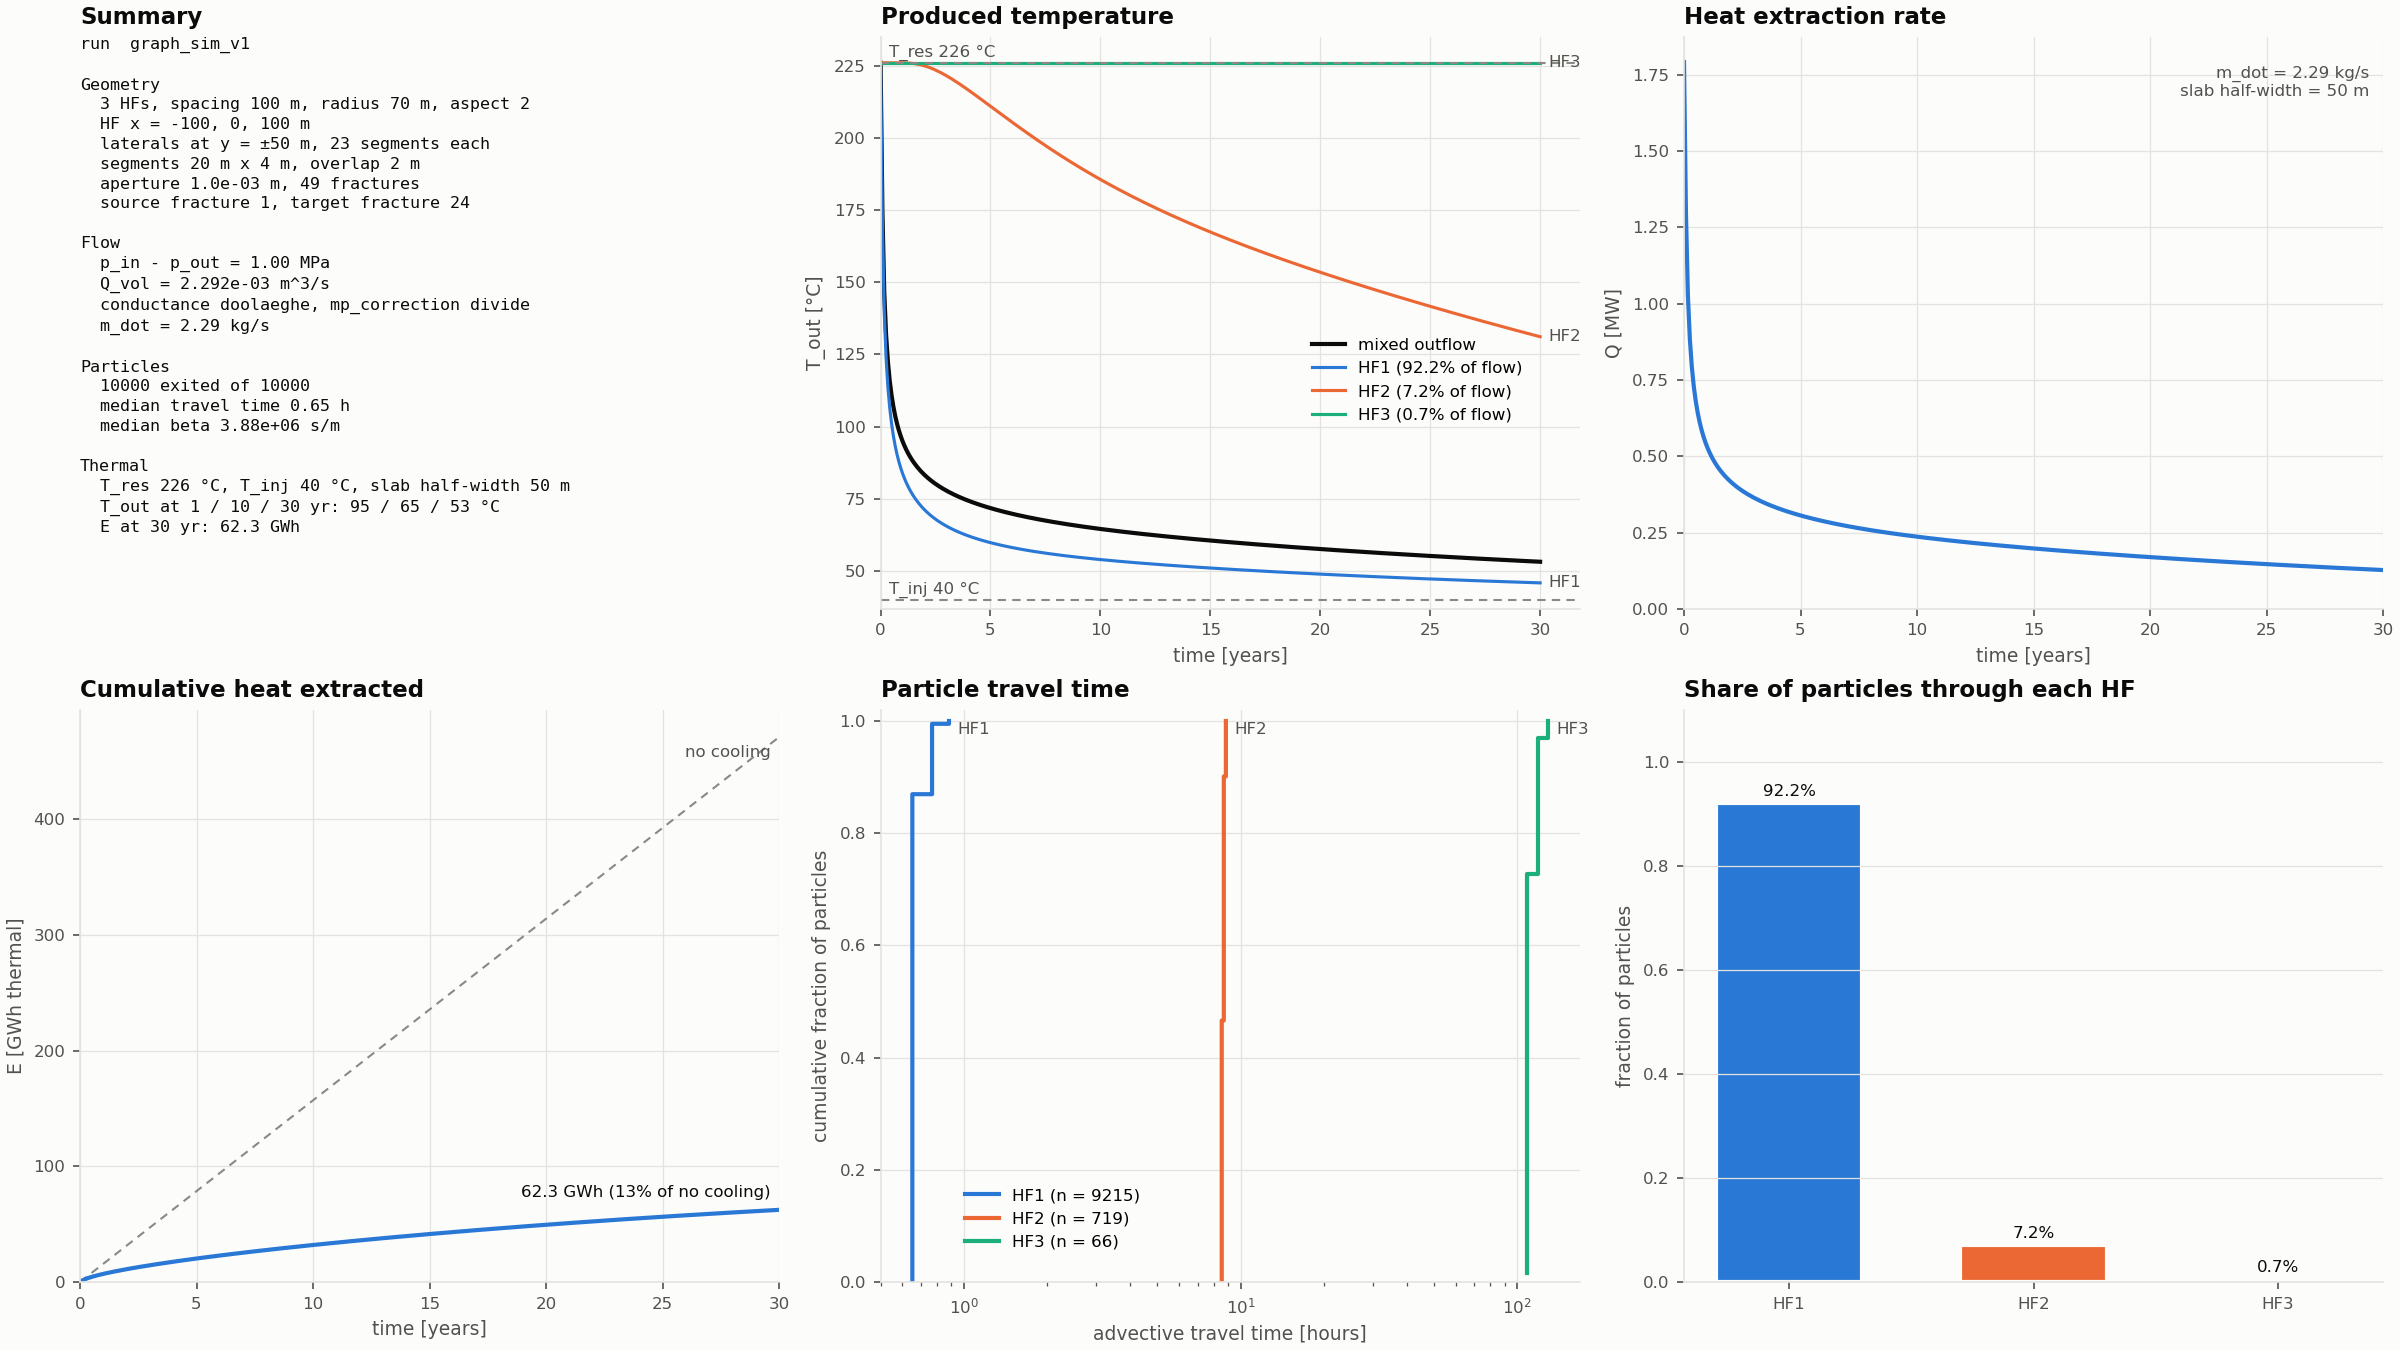
\includegraphics[height=0.84\textheight]{figs/results.png}
\note{The driver\_v1 configuration after all fixes. The mass flow rate is 2.29 kg/s at a 1 MPa pressure drop. 92 percent of particles take the HF nearest the well ends, HF1, with travel times under an hour; 7 percent take HF2 and under 1 percent HF3. The mixed outflow therefore follows HF1: 95 C after one year, 65 C after ten and 53 C after thirty. Heat rate starts at 1.8 MW and falls to 0.13 MW. Over thirty years 62 GWh are extracted, 13 percent of what the same flow would give with no cooling.}
\end{frame}

% ------------------------------------------------------------------
\begin{frame}{Before and after the fixes (same geometry, HF aspect 1)}
\centering
\includegraphics[width=0.8\textwidth]{figs/before_after.pdf}

\footnotesize
\begin{tabular}{@{}lccc@{}}
\toprule
 & $\dot m$ [kg/s] & $T_\mathrm{out}$ at 1 / 10 / 30 yr [$^\circ$C] & $E$ at 30 yr [GWh] \\
\midrule
before & 0.92 & 99 / 63 / 51 & 23 \\
after  & 2.28 & 93 / 63 / 52 & 59 \\
\bottomrule
\end{tabular}
\note{Same geometry, HF aspect 1, before and after the three fixes. The produced temperature barely moves: the flow-equivalent width raises the rock contact per edge, but the flow rate through it rises too, and the two nearly cancel in beta. The mass flow rate is 2.5 times higher, because the flows now follow the Doolaeghe conductances instead of the narrow Karra strips, so the heat extracted over thirty years goes from 23 to 59 GWh. Temperature alone would have hidden the change.}
\end{frame}

% ------------------------------------------------------------------
\begin{frame}{Interpretation and caveats}
\begin{itemize}
  \item \textbf{Short circuit}: 92\% of the flow takes HF1, the HF nearest the well ends; HF2 and HF3 are nearly idle.
  \item \textbf{Cooling is fast} because HF1's contact area is small for its flow: $2 L W \approx 2\times100\times41$\,m$^2$ at about 2\,kg/s, so $t_s\approx0.2$\,yr.
  \item \textbf{Flow-equivalent width $\neq$ swept width}: the conductance is dominated by convergence at the 4\,m well intersections, while the heat sees the whole area the flow sweeps; for dipole flow in a 140\,m $\times$ 280\,m HF that area is larger.
  \item \textbf{Model assumptions}: steady flow; rock initially at $T_\mathrm{res}$; conduction only normal to the walls; independent particles; one slab half-width $B$ for every HF.
\end{itemize}
\note{The geometry sends almost all the flow through the HF nearest the well ends, so the result is essentially one fracture's cooling. That fracture cools within a year or two because its rock contact is small for the flow it carries. The flow-equivalent width is consistent with the flow model, but it is a hydraulic width: the conductance is controlled by flow converging onto short well intersections. The heat exchange depends on the area the flow actually sweeps, which for dipole flow between two wells in a large fracture is wider. That is the main open modelling question and the first item on the next slide.}
\end{frame}

% ------------------------------------------------------------------
\begin{frame}{Next steps}
\begin{enumerate}
  \item \textbf{YAML files controlling the runs}: geometry, flow, transport and thermal inputs per run; driver reads one file.
  \item \textbf{Swept-area check}: compare the flow-equivalent width with a whole-fracture sweep ($2A_f/Q_f$ per fracture) as an upper bound on rock contact.
  \item \textbf{Fixed rate}: solve at a target $\dot m$ instead of a fixed pressure drop, so runs are comparable.
  \item \textbf{Stochastic background}: natural fracture sets around the HFs; spacing and connectivity sweeps.
  \item \textbf{Validation}: one case against a meshed PFLOTRAN or FEHM thermal run.
  \item \textbf{dfnWorks}: move the well and thermal helpers into \texttt{pydfnworks} once the interface settles.
\end{enumerate}
\note{Next: put every run's inputs in a YAML file the driver reads, so cases are reproducible and easy to sweep. Then bound the rock-contact question by comparing with a whole-fracture sweep. Imposing a target mass flow rate makes runs with different geometry comparable. After that, add the stochastic background network and sweep spacing and connectivity, validate one case against a meshed thermal simulation, and move the helpers into pydfnworks.}
\end{frame}

\end{document}
